\documentclass[xcolor=pdftex,dvipsnames,table,mathserif,aspectratio=169]{beamer}
\usetheme{default}
%\usetheme{Darmstadt}
%\usepackage{times}
%\usefonttheme{structurebold}

\usepackage[english]{babel}
%\usepackage[table]{xcolor}
\usepackage{pgf,pgfarrows,pgfnodes,pgfautomata,pgfheaps}
\usepackage{amsmath,amssymb,setspace}
\usepackage[latin1]{inputenc}
\usepackage[T1]{fontenc}
\usepackage{relsize}
\usepackage[absolute,overlay]{textpos} 
\newenvironment{reference}[2]{% 
  \begin{textblock*}{\textwidth}(#1,#2) 
      \footnotesize\it\bgroup\color{red!50!black}}{\egroup\end{textblock*}} 

\DeclareMathSizes{10}{10}{6}{6} 


\title [Single-agent dynamic optimization models]{Persistent Unobservables}
\author{C.Conlon - Adapted from M. Shum}
\institute{Grad IO}
\date{\today}
\setbeamerfont{equation}{size=\tiny}
\begin{document}


\begin{frame}
\titlepage
\end{frame}


\begin{frame}
From Shepard (2015 JMP):
\begin{itemize}
\item Wants to measure the impact of ``star hospitals''.
\item Previous wisdom was that in MA you needed to include Partners Healthcare in your insurer's network.
\item From 2010-2012 Harvard Pilgrim (\#2) insurer excluded Partners Hospital Network (MGH, Brigham Womens, Harvard-MIT teaching hospitals) from their plan
\begin{itemize}
\item Comparable procedures are around 40\% more expensive at Partners' Hospitals
\item Customers revolted! Employer sponsored left in droves, strikes, etc.
\item Can't run a network without them.
\end{itemize}
\item With the ACA it looks like nobody wants to have Partners in their network anymore.
\item Consumers face same prices for all hospitals
\item Idea: two dimensions of heterogeneity. 
\begin{itemize}
\item Some people like option of MGH in case they get really sick (rare cancer)
\item Others go to MGH because they have doctors there, have gone in the past, or enjoy amenities but could get comparable care elsewhere.
\end{itemize}
\end{itemize}
\end{frame}



\begin{frame}{Persistence: Reduced form proxy}
From Shepard (2015 JMP):
\begin{center}
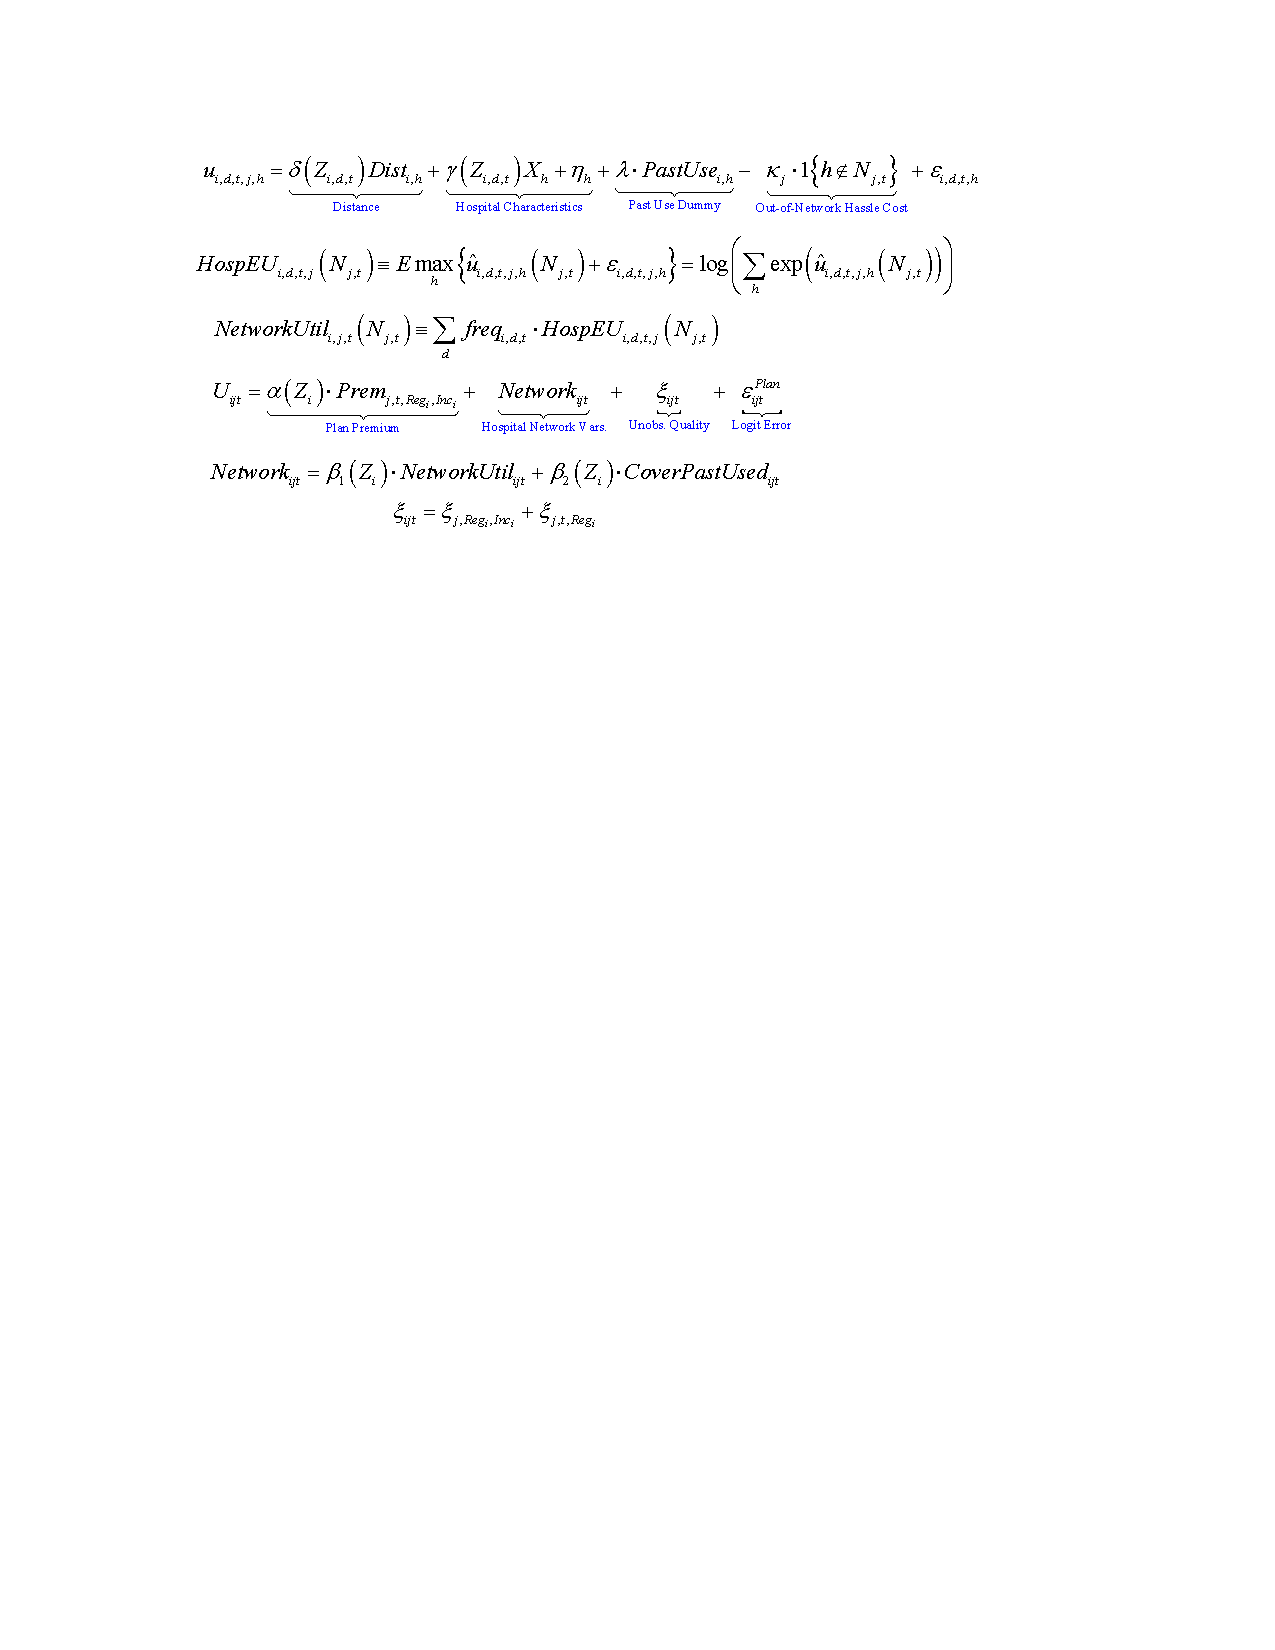
\includegraphics[width=4.5in]{resources/shepardsized}
\end{center}
\end{frame}


\begin{frame}{Unobserved State Variables}
\begin{itemize}
\item Up until now we consider models satisfying Rust's \alert{conditional independence} assumption on the $\varepsilon$'s. This rules out persistence in unobservables which are economically meaningful.
\item Suppose there are two types of buses good $(s_i=g)$ and bad $(s_i=b)$.
\item Assume that this is known to HZ but not the econometrician.
\item Single period utility now depends on $\alert{s_i}$ so $u(x_{it},s_i,d_{it}; \theta)$ \alert{unobserved state variable}.
\item In case of the nested fixed point algorithm, this unobserved persistent heterogeneity is not a big problem as we can solve for the value function (and expected policy functions) given the state variables and \alert{integrate it out} in the likelihood
\end{itemize}
\end{frame}



\begin{frame}{Unobserved State Variables}
\begin{eqnarray*}
p(y | x) &=& \int p(y | x, s) p(s) \\
Pr(d_{it} = 1|x_{it}) &=& Pr(s_i = 1)�Pr(d_{it} = 1|x_{it},s_i = 1) \\
&+&Pr(s_i = 0)�Pr(d_{it} = 1|x_{it},s_i = 0)
\end{eqnarray*}
Note that the unobserved $s_i$ generates correlation in decisions over time for a given bus. Therefore, the likelihood of a sequence of decisions for a given bus must be integrated over $s$\begin{eqnarray*}
\tiny
Pr(d_{i1},\ldots,d_{iT} | x_{i1},\ldots,x_{iT} )&=& \sum_{s} Pr(d_{i1},\ldots,d_{iT} | x_{i1},\ldots,x_{iT} )  p(s_i) \\
Pr(d_{i1},\ldots,d_{iT} | x_{i1},\ldots,x_{iT} ) &=& \sum_{s}  \prod_{t=1}^T Pr(d_{it} | x_{it} )  p(s_i) \\
\end{eqnarray*}
\alert{Conditional on $s_i$ replacement decisions are independent across $t$ given $x_{it}$}.

\end{frame}


\begin{frame}{Single-agent dynamics part 3}
Up until now we consider models satisfying Rust's \textit{conditional independence} assumption on the $\varepsilon$'s. This rules out persistence in unobservables which are economically meaningful.\\
\vspace{0.5cm}
\textbf{Pakes (1986): Patents as Options}: How much are patents worth? Valuable for optimal patent length and design? Sufficient incentive for innovation?
\begin{itemize}
\item $Q_A$: value of patent at age $A$
\item Goal of paper is to estimate $Q_A$ using data on their renewal. $Q_A$ is  inferred from patent renewal process via \textit{structural model} of patent renewal behavior.
\item Treat renewal systems as exogenous (in Europe)
\item For $a=1,\ldots,L$ a patent can be renewed by paying the fee $c_a$.
\end{itemize}
\end{frame}


\begin{frame}{Pakes (1986)}
Timing
\begin{itemize}
\item At age $a=1$ patent holder gets $r_1$ from patent
\item Decide whether or not to renew (pay $c_1$ and go to $a_2$).
\item At age $a=2$ get $r_2$ from patent
\item and so on...
\end{itemize}
Gives us the value function
\begin{eqnarray*}
V&\equiv& \max_{t \in [a,L] }\sum_{a'=1}^{L-a} \beta^{a'} R(a+ a') \\
R(a) &=& \begin{cases} r_a -c_a, & \mbox{if } t \geq a \mbox{ when you hold patent} \\0 & \mbox{if } t < a \mbox{ after patent expires} \end{cases}
\end{eqnarray*}
$t$ above denotes the age which allows the patent to expire and is the choice variable.  This is an \textit{optimal stopping} problem.\\

$R(a)$ are the profits from year $a$.  This is a \textit{controlled} stochastic process.  It is random but affected by the actions of the agent.
\end{frame}


\begin{frame}{Pakes (1986)}
\begin{itemize}
\item The maximum age $L$ is finite so it is finite-horizon DP.
\item The single period revenue $r_a$ is the state variable.
\item We can solve the problem with \textit{backward recursion}.
\end{itemize}
\begin{eqnarray*}
V_a(r_a) = \max  \left\{0, Q_a \equiv r_a + \beta E[V_{a+1} (r_{a+1} ) | \Omega_a] - c_a  \right\}
\end{eqnarray*}
\vspace{-0.75cm}
\begin{itemize}
\item Renew iff $Q_a - c_a > 0$.
\item $\Omega_a$: history up to age $a = \{r_1,r_2,\ldots,r_a\}$.
\item Expectation is over $r_{a+1} | \Omega_{a}$. The sequence of conditional distributions $G_a \equiv F(r_{a+1} | \Omega_a)$, $a=1,2,\ldots$ is an important component of model specification.
\begin{eqnarray*}
r_{a+1} = \begin{cases} 0  & \mbox{w. prob } \exp(-\theta r_a) \\
\max(\delta r_a,z) & \mbox{w. prob } 1-\exp(-\theta r_a) \end{cases}
\end{eqnarray*}
\end{itemize}
\end{frame}


\begin{frame}{Pakes (1986)}
Model has the following parameters
\begin{itemize}
\item density of $z$ $q_a = \frac{1}{\sigma_a} \exp[-(\gamma+z)/\sigma_a]$ and $\sigma_a = \phi^{a-1} \sigma$, for $a=1,\ldots,L-1$. 
\item $(\delta, \theta, \gamma, \phi, \sigma)$ are the structural parameters of the model
\item Break down the model period by period and decide whether or not to renew if $Q_a = r_a + $ ``option value''.
\item Option value is about keeping the patent alive in case it pays off in the future.
\end{itemize}
Implications
\begin{itemize}
\item Drop out at age $a$ if $c_a > Q_a$
\item Optimal decision is characterized by cutoff points $Q_a > c_a \Leftrightarrow r_a > \overline{r}_a$  (Key assumptions is $Q_a$ increasing /single crossing )
\item Cutoff points are increasing sequence $\overline{r}_{a} < \overline{r}_{a+1} < \ldots < \overline{r}_{L-1}$.
\end{itemize}
\end{frame}


\begin{frame}{Estimation}
Instead of using Pakes' notation $r_t$ for the patent revenue. We will use the generic Rust notation of $\epsilon_t$ the unobserved state variable, and $i_t$ to denote the choice (renewal).
\begin{itemize}
\item For a single patent $\tilde{T}$ denotes the age at which it is allowed to expire. Let $T = \min(L-1,\tilde{T})$ denote the period sins which the agent makes a renewal decision where we model the agent's choice.
\item $\epsilon$ follows a first-order Markov process $F(\epsilon' | \epsilon)$
\item Age-specific policy function by $i^*_t(\epsilon)$.
\end{itemize}
Likelihood function is 
\begin{eqnarray*}
l(i_1,\ldots,i_T | \epsilon_0,i_0,\theta) = \prod_{t=1}^T Prob(i_t | i_0, \ldots,  x_{t-1}, i_{t-1} ; \epsilon_0, \theta)
\end{eqnarray*}
Serial correlation in $\epsilon$ means there is dependence among $i_{t}, i_{t-2}$ even after conditioning on $x_{t-1},i_{t-1}$. 
\end{frame}

\begin{frame}{Simulation}
\begin{itemize}
\item It might seem like we were stuck since it no longer has a closed form.  However, we can simulate the ``outer loop'' of the nested fixed point routine given a guess  of $i^*_t(\epsilon,\theta)$.
\item Because $\epsilon$ is serially correlated we need to start with an initial $\epsilon_0$ (or distribution) and assume that it is known.  This is the \textit{initial conditions problem} of finite MDPs.
\item Note that simulation is part of the ``outer loop'' of nested fixed point estimation routine. So at the point when we simulate, we already know the policy functions $i_t^{*}(\epsilon,\theta)$ (How would you compute this?)
\end{itemize}
\end{frame}

\begin{frame}{Naive Frequency Simulator (Don't do this...)}
Go back to the full likelihood function (condition on initial $\epsilon_0$ for serial correlation):
\begin{eqnarray*}
l(i_1,\ldots,i_T | i_0, \epsilon_0, \theta) = Pr(i_t^{*} (\epsilon_t,\theta) = i_t, \forall t =1,\ldots,T)
\end{eqnarray*}
Need to take probability over distribution of $(\epsilon_1,\ldots,\epsilon_T | \epsilon_0)$.  Let $F(\epsilon_{t+1} | \epsilon_t,\theta)$ then the above probability can be expressed as the integral:
\begin{eqnarray*}
\int \cdots \int \prod_t \mathbf{1}(i_t^{*}(\epsilon_t,\theta) = i_t) \prod_t d F(\epsilon_t | \epsilon_{t-1}; \theta)
\end{eqnarray*}
Simulate by drawing sequences of $(\epsilon_t)$.
\end{frame}

\begin{frame}{Naive Frequency Simulator (Don't do this...)}
Simulate by drawing sequences of $(\epsilon_t)$ and for each draw $s=1,\ldots,S$ we take as initial values $(x_0,i_0,\epsilon_0)$ then
\begin{itemize}
\item Generate $(\epsilon_1^s, i_1^s)$
	\begin{enumerate}
	\item Generate $\epsilon_1^s \sim F(\epsilon_1 | \epsilon_0)$ 
	\item Compute $i_1^s = i_1^{*}(\epsilon_1^s; \theta)$
	\end{enumerate}
\item Generate $(\epsilon_2^s, i_2^s)$
	\begin{enumerate}
	\item Generate $\epsilon_2^s \sim F(\epsilon_2 | \epsilon_1^s)$ 
	\item Subsequently compute $i_2^s = i_2^{*}(\epsilon_2^s; \theta)$
	\end{enumerate}
\item And so on, up to $(\epsilon_T^s,i_T^s)$.
\end{itemize}
And for the case where $(i,x)$ are both discrete (Rust) we can approximate:
\vspace{-0.5cm}
\begin{eqnarray*}
l(i_t,\ldots,i_T | \epsilon_0,i_0;\theta) \approx \frac{1}{S} \sum_s \prod_{t=1}^T \mathbf{1}(i_t^s = i_t)
\end{eqnarray*}
Frequency of simulated sequences which match observed sequence.  $T$ long or $S$ small you're in trouble (non-smooth).
\end{frame}

\begin{frame}{Importance Sampling: Particle Filtering}
\begin{itemize}
\item We can use importance sampling to simulate the likelihood function. 
\item This is not straightforward given time dependence in $(i_t,\epsilon_t)$
\item Consider particle filtering approach from Fernandez-Villaverde and Rubio-Ramirez (2007) or Flury and Shehard (2008) (non-Gaussian Kalman filtering).
\end{itemize}
\end{frame}

\begin{frame}{Importance Sampling: Particle Filtering}
\begin{itemize}
\item Evolution of utility shocks $\epsilon_t | \epsilon_{t-1} \sim f(\epsilon' | \epsilon)$. Ignore dependence of distribution of $\epsilon$ on age $t$ for convenience.
\item As before, the policy function is $i_t = i^{*}(\epsilon_t)$
\item Let $\epsilon^t \equiv \{\epsilon_1,\ldots,\epsilon_t\}$.
\item The initial values of $y_0$ and $\epsilon_0$ are known
\end{itemize}
Go back to the factorized likelihood
\begin{eqnarray*}
l(y^T | y_0,\epsilon_0 ) &=& \prod_{t=1}^T l (y_t | y^{t-1},y_0,\epsilon_0) = \prod_{t=1} \int l (y_t |\epsilon^t, y^{t-1}) p(\epsilon^t | y^{t-1} )d \epsilon^t  \\
&\approx& \frac{1}{S} \sum_s l(y_t | \epsilon^{t | t-1,s},y^{t-1})
\end{eqnarray*}
We omit conditioning on $(\epsilon_0, y_0)$ for convenience, and $\epsilon^{t | t-1,s}$ is a simulated draw of $\epsilon^t \sim p(\epsilon^t | y^{t-1})$.
\end{frame}



\begin{frame}{Importance Sampling: Particle Filtering}
Let's look more closely at the last line:
\begin{itemize}
\item first term: $l(y_t, | \epsilon^t,y^{t-1})$ we can calculate for a value of $\epsilon_t$
\begin{eqnarray*}
l(y_t | \epsilon^t , y^{t-1}) = p(i_t | \epsilon^t, y^{t-1}) = p(i_t | \epsilon_t) = \mathbf{1}(i(\epsilon_t) = i_t)
\end{eqnarray*}
\item the second term $p(\epsilon^t | y^{t-1})$ is generally not obtainable in closed form. So numerical integration is not feasible. Particle filtering let's us draw $\epsilon^t$ from this distribution for every period $t$.
\end{itemize}
Particle filtering proposes a recursive approach to draw sequences $p(\epsilon^t | y^{t-1})$ for every $t$
\end{frame}


\begin{frame}{Particle Filtering Algorithm}
\textbf{First period:} $t=1$ In order to simulate the integral corresponding to the first period we need to draw from $p(\epsilon^1 | y^0,\epsilon_0)$ (easy).  
\begin{itemize}
\item We draw $\{\epsilon^{1|0,s }\}_{s=1}^S$ according to $f(\epsilon' | \epsilon_0)$.
\item The notation $\epsilon^{1|0,s}$ makes it explicit that the $\epsilon$ is a draw from $p(\epsilon^1 | y^0,\epsilon_0)$
\item Use the $S$ draws we can evaluate the period $t=1$ likelihood.
\end{itemize}
\textbf{Second period:} $t=2$. We need to draw from $p(\epsilon^2 | y^1)$ factorize as:
\begin{eqnarray*}
p(\epsilon^2 | y^1) = p(\epsilon^1 | y^1) \cdot p(\epsilon_2 | \epsilon^1) \mbox{ recall } \epsilon^2 \equiv \{\epsilon_1,\epsilon_2\}
\end{eqnarray*}
\end{frame}

\begin{frame}{Filtering Step}
Getting a draw from $p(\epsilon^1| y^1)$, given that we already have draws $\{\epsilon^{1|0,s} \}$ from $p(\epsilon^1 | y_0)$, from the previous period $t = 1$, is the heart of particle filtering. We use the principle of importance sampling: by Bayes' Rule
\begin{eqnarray*}
p(\epsilon^1 | y^1) \propto p(y_1 | \epsilon^1, y^0) \cdot p (\epsilon^1 | y^0)
\end{eqnarray*}
Hence, if our desired sampling density is $p(\epsilon^1 | y^1)$, but we actually have draws $\{ \epsilon^{1|0,s}\}$ from $p(\epsilon^1| y^0)$, then the importance sampling weight for the draw
 $\epsilon^{1|0,s}$ is proportional to
\begin{eqnarray*}
\tau_1^s \equiv p(y_1 | \epsilon^{1|0,s},y^0)
\end{eqnarray*}
Note that this coincides with the likelihood contribution for period 1, evaluated at the shock $\epsilon^{1|0,s}$.The SIR algorithm in Rubin (1988) proposes that making $S$ draws with replacement from samples $\{ \epsilon^{1|0,s}\}_{s=1}^S$, using weights proportional $\tau_1^s$ yields draws from the desired density $p(\epsilon^1 | y^1)$ which we denote $\{ \epsilon^{1|0,s}\}_{s=1}^S$.
\end{frame}

\begin{frame}{Prediction Step}
For the second term in the equation: we simply draw one $\epsilon_2^s$ from $f(\epsilon' | \epsilon^{1,s})$, for each draw $\epsilon^{1,s}$ from the filtering step. This is the \textbf{prediction} step.\\
\vspace{0.25cm}
By combining the draws from these two terms, we have $\{ \epsilon^{2|1,s}\}_{s=1}^S$.which is $S$ drawn sequences from $p(\epsilon^2 | y^1)$. Using these $S$ draws, we can evaluate the simulated likelihood for period 2.\\

\vspace{0.25cm}
\textbf{Third period, $t = 3$:} start again by factoring
\begin{eqnarray*}
p(\epsilon^3 | y^2) = p(\epsilon^2 | y^2) \cdot p(\epsilon_3 | \epsilon^2)
\end{eqnarray*}
As above, drawing from  requires filtering the draws $\{ \epsilon^{2|1,s}\}_{s=1}^S$, from the previous period $t = 2$, to obtain draws $\{ \epsilon^{2,s}\}_{s=1}^S$. Given these draws, draw $\epsilon_3^s \sim f(\epsilon' | \epsilon^{2,s})$ for each $s$.\\

And so on. By the last period $t = T$, you have
\begin{eqnarray*}
\left\{ \{ \epsilon^{t|t-1,s}\}_{s=1}^S \right\}_{t=1}^T
\end{eqnarray*}
\end{frame}

\begin{frame}{Prediction Step (continued)}
Hence the factorized likelihood can be approximated by simulation as:
\begin{eqnarray*}
\prod_t \frac{1}{S} \sum_s l (y_t | \epsilon^{t|t-1,s},y^{t-1})
\end{eqnarray*}
As noted above, the likelihood term $l(y_t | \epsilon^{t | t-1,s},y^{t-1})$ coincides with the simulation weight $\tau_t^s$. Hence the simulated likelihood can also be constructed as:
\begin{eqnarray*}
\log l (y^T | y_0, \epsilon_0) = \sum_t \log \left\{ \frac{1}{S} \sum_s \tau_t^s \right\}
\end{eqnarray*}
\end{frame}

\begin{frame}{Particle Filtering (Summary)}
\begin{itemize}
\item Start by drawing $\{ \epsilon^{1|0,s}\}_{s=1}^S$ from $p(\epsilon^1 | y^0, \epsilon_0)$.
\item In period $t$, we start with $\{ \epsilon^{t-1|t-2,s}\}_{s=1}^S$ draws from $p(\epsilon^{t-1} | y^{t-2},\epsilon_0)$.
\begin{enumerate}
\item \textbf{Filter step:} Calculate proportion weights $\tau_{t-1}^s \equiv p(y_{t-1} | \epsilon^{t-1 | t-2,s}, y^{t-2}) $ using $p(i_t | \epsilon_t)$. Draw$\{\epsilon^{t-1 | t-1,s}\}_{s=1}^S$ by resampling from $\{ \epsilon^{t-1|t-2,s}\}_{s=1}^S$ with weights $\tau_{t-1}^s$.
\item \textbf{Prediction step:} Draw $\epsilon_t^s$ from $p(\epsilon_t | \epsilon^{t-1 | t-1,s})$ , for $s=1,\ldots,S$. Combine to get 
$\{ \epsilon^{t | t-1,s} \}_{s=1}^S$.
\end{enumerate}
\item Set $t=t+1$ and go back to step 2.  Stop when $t=T+1$.
\end{itemize}
The difference is that the crude simulator draws $S$ sequences and puts zero weight on those which don't match the observed sequin. In each period $t$ we just keep sequences where predicted choices match observed choice of \textit{that period}. This is more accurate likelihood as long as $S$ is large enough that we don't have all the weight on a single sequence in period $t$.
\end{frame}


\begin{frame}{References}
\begin{itemize}
\item Fernandez-Villaverde, J., and J. Rubio-Ramirez (2007): ``Estimating Macroeco- nomic Models: A Likelihood Approach,'' Review of Economic Studies, 74, 1059-1087.\\
\item Flury, T., and N. Shephard (2008): ``Bayesian inference based only on simulated likelihood: particle filter analysis of dynamic economic models,'' manuscript, Oxford University\\
\item Pakes, A. (1986): ``Patents as Options: Some Estimates of the Value of Holding European Patent Stocks,'' Econometrica, 54(4), 755-84.\\
\item Rubin, D. (1988): ``Using the SIR Algorithm to Simulate Posterior Distributions,'' in Bayesian Statistics 3, ed. by J. Bernardo, M. DeGroot, D. Lindley, and A. Smith. Oxford University Press.\\
\end{itemize}
\end{frame}


\end{document}














































